\documentclass[11pt]{article}
\usepackage{ctex} %中文
\usepackage[utf8]{inputenc}
\usepackage[a4paper, left=3cm, right=3cm, top=2.5cm, bottom=2.5cm]{geometry} 

\usepackage{graphicx}
\usepackage{subcaption}
\usepackage{float}
\usepackage{amsmath, amsthm, amssymb}

%代码块格式
\usepackage{listings}
\usepackage{xcolor} %设置颜色
%\usepackage{setspace} % 用于调整行间距

%\usepackage{parskip}  

\usepackage{booktabs} %精美表格

% 定义代码样式：
\lstset{
    language=Python,
    basicstyle=\ttfamily\small,
    %numbers=left,
    numberstyle=\tiny\color{gray},
    stepnumber=1,
    breaklines=true,
    frame=shadowbox,
    commentstyle=\color{green!60!black},
    keywordstyle=\color{blue},
    stringstyle=\color{purple},
    backgroundcolor=\color{white},
    showstringspaces=false,
    showspaces=false
}
\title{\textbf{Homework of Chapter 5}}
\author{Name: Kaifeng Tang \quad ID: 524030910124}
\date{\today}

\begin{document}
\maketitle 
\section*{简答题}
\subsection*{1. } 
距离向量算法核心：Bellman-Ford方程\[D_x(y) = \min_v \{c(x, v) + D_v(y)\}\]

其中$D_x(y)$为从x到y的最小路径代价。

对于节点z，初始化$D_z(z) = 0, D_z(v) = 6, D_z(x) = 2$。
先初始化距离表：
\begin{table}[!htbp]
    \centering
    \renewcommand{\arraystretch}{1.3}
    \begin{tabular}{c c c c c c}
        \toprule
        起点/终点 & u & v & x & y & z \\
        \midrule
        u & 0 & 1 & $\infty$ & 2 & $\infty$ \\
        v & 1 & 0 & 3 & $\infty$ & 6 \\
        x & $\infty$ & 3 & 0 & 3 & 2 \\
        y & 2 & $\infty$ & 3 & 0 & $\infty$ \\
        z & $\infty$ & 6 & 2 & $\infty$ & 0 \\
        \bottomrule
    \end{tabular}
\end{table}

由BF方程开始更新：
\[D_z(u) = \min\{c(z, v)+D_v(u), c(z,x)+D_x(u)\} = 7\]

同理， 
\[D_z(v) = 5, D_z(x) = 2, D_z(y) = 5, D_z(z) = 0\]

不断更新直到所有节点距离向量稳定，最终得到节点z的距离表：
\begin{table}[!htbp]
    \centering
    \renewcommand{\arraystretch}{1.3}
    \begin{tabular}{c c c c c c}
        \toprule
        z/终点 & u & v & x & y & z \\
        \midrule
        z & 6 & 5 & 2 & 5 & 0 \\
        \bottomrule
    \end{tabular}
\end{table}

\subsection*{2. }
由Dijkstra算法，初始化集合$N'={t}$；对所有t的邻居，$D(v) = c(t, v)$；其余令$D(v) = \infty$.
然后进行如下循环：
\begin{itemize}
    \item 在集合$N'$以外找到$D(w)$的最小值对应的节点w
    \item 将w加入集合$N'$
    \item 对于w的不在$N'$里的邻居进行更新：$D(v) = \min\{D(v), D(w) + c(w, v)\}$ 
\end{itemize}

直到所有节点都加入$N'$，即可得到t到其他节点的最短路径。
用填表法一步步更新，最终得到下面的表。
\begin{table}[!htbp]
    \centering
    \renewcommand{\arraystretch}{1.2}
    \begin{tabular}{c c c c c c c c c}
        \toprule
        Step & $N'$ & D(u),p(u) & D(v),p(v) & D(w),p(w) & D(x),p(x) & D(y),p(y) & D(z),p(z) \\
        \midrule
        0 & t & 2,t & 4,t & $\infty$ & $\infty$ & 7,t & $\infty$ \\
        1 & tu & & 4,t & 5,u & $\infty$ & 7,t & $\infty$ \\
        2 & tuv & & & 5,u & 7,v & 7,t & $\infty$ \\
        3 & tuvw & & & & 7,v & 7,t & $\infty$ \\
        4 & tuvwy & & & & 7,v & & 19,y \\
        5 & tuvwyx & & & & & & 15,y \\
        6 & tuvwyxz & & & & & & \\
        \bottomrule
    \end{tabular}
\end{table}

$tuvwyxz$即为最小代价生成树，表征t到各节点的最短路径；同时可以得到节点t到各节点的最短路径长度：
\begin{table}[!htbp]
    \centering
    \renewcommand{\arraystretch}{1.2}
    \begin{tabular}{c c c c c c c c}
        \toprule
        节点 & u & v & w & x & y & z \\
        \midrule
        $Dist_t$ & 2 & 4 & 5 & 7 & 7 & 15 \\
        \bottomrule
    \end{tabular}
\end{table}

\subsection*{3. }
\textbf{1) }BGP 路由选择会基于策略控制。一般商业策略中，AS 会更倾向于使用成本更低或收益更高的路径。
由于经过 provider 发送流量通常需要付费，而 peer 之间交换流量成本较低，因此
当 AS100 同时从 AS200 和 AS300 收到到达同一目的网络的路由通告时，通常会优先选择 AS300 这条 peer 路径。

\textbf{2) }transit-AS 意味着 AS100 不仅转发自己产生或发往自己的流量，还允许其他 AS 的流量经过 AS100 转发到第三方 AS。
则需要调整策略：
\begin{itemize}
    \item AS100 不仅通告自己的路由，还可能把从 AS300 学到的路由通告给 AS200，把从 AS200 学到的路由通告给 AS300。
    \item 允许将 peer 学到的路由与provider路由相互通告。
    \item 调整本地偏好和路由过滤策略。
\end{itemize}

可能存在的风险：带宽压力增加，导致链路拥塞；运营成本增加；
可能会有安全风险如 DDoS、扫描、攻击流量等安全问题；
路由策略复杂度变高。

\qquad

\section*{Lab5 基于RIP的路由配置实验}
\subsection*{1. 实验目的}
本实验基于 Ubuntu 虚拟机中的 Mininet 与 FRR 软件完成 RIP 动态路由配置。
通过构建包含 R1、R2、R3、R4、R5 五台路由器的网络拓扑，观察 RIP 协议在正常状态、链路故障状态以及链路恢复状态下的路由表变化，
理解距离向量路由协议的基本工作原理、路由收敛过程以及链路故障后的动态路由更新机制。

\subsection*{2. 实验过程及分析}
\subsubsection*{(1) 搭建实验拓扑}
本实验使用 5 台路由器节点。由实验要求的链路关系图，可以设置各链路的对应网段，如下表所示。
每台路由器通过 FRR 的 zebra 和 ripd 进程运行 RIP 协议，并在各自的配置文件中声明自身的直连网段，使路由器之间能够交换路由信息。
\begin{table}[!htbp]
    \centering
    \renewcommand{\arraystretch}{1.0}
    \begin{tabular}{c c c}
        \toprule
        链路 & \quad 对应网段 & 接口ip \\
        \midrule
        R1-R2 &	\qquad 10.0.1.0/24	& \qquad R1: 10.0.1.1，R2: 10.0.1.2 \\
        R2-R3 &	\qquad 10.0.2.0/24	& \qquad R2: 10.0.2.1，R3: 10.0.2.2 \\
        R4-R5 &	\qquad 10.0.3.0/24	& \qquad R4: 10.0.3.1，R5: 10.0.3.2 \\
        R1-R4 &	\qquad 10.0.4.0/24	& \qquad R1: 10.0.4.1，R4: 10.0.4.2 \\
        R2-R5 & \qquad 10.0.5.0/24	& \qquad R2: 10.0.5.1，R5: 10.0.5.2 \\
        R3-R5 & \qquad 10.0.6.0/24	& \qquad R3: 10.0.6.1，R5: 10.0.6.2\\
        \bottomrule
    \end{tabular}
\end{table}

由示例代码编写实验拓扑运行脚本\texttt{rip\_lab.py}.

\subsubsection*{(2) 启动拓扑}
运行拓扑脚本，进入mininet环境，并等待RIP 协议完成初始收敛。
随后分别查看 R1、R2、R3、R4、R5 的 ip route 路由表，如图1所示。

从初始化路由表截图可以看到，每台路由器的路由表中均包含两类路由：
\begin{itemize}
    \item \texttt{proto kernel}, 表示该路由器的直连路由，由系统根据接口 IP 自动生成。
    \item \texttt{proto rip}, 表示该路由器通过 RIP 协议动态学习到的非直连网段路由。
\end{itemize}
例如在R1 的路由表中，直连路由为：
\begin{lstlisting}
10.0.1.0/24 dev r1-eth0 proto kernel
10.0.4.0/24 dev r1-eth1 proto kernel
\end{lstlisting}
同时，R1还通过RIP协议学习到其他的RIP非直连路由：
\begin{lstlisting}
10.0.2.0/24 via 10.0.1.2 dev r1-eth0 proto rip
10.0.3.0/24 via 10.0.4.2 dev r1-eth1 proto rip
10.0.5.0/24 via 10.0.1.2 dev r1-eth0 proto rip
10.0.6.0/24 via 10.0.1.2 dev r1-eth0 proto rip
\end{lstlisting}

这说明R1 已经通过 RIP 协议学习到了 R2-R3、R4-R5、R2-R5、R3-R5 等非直连网段的路由信息。
对R2~R5的分析同理。由此可以判断，初始状态下 RIP 已经完成路由收敛。

\begin{figure}[!htbp]
    \centering
    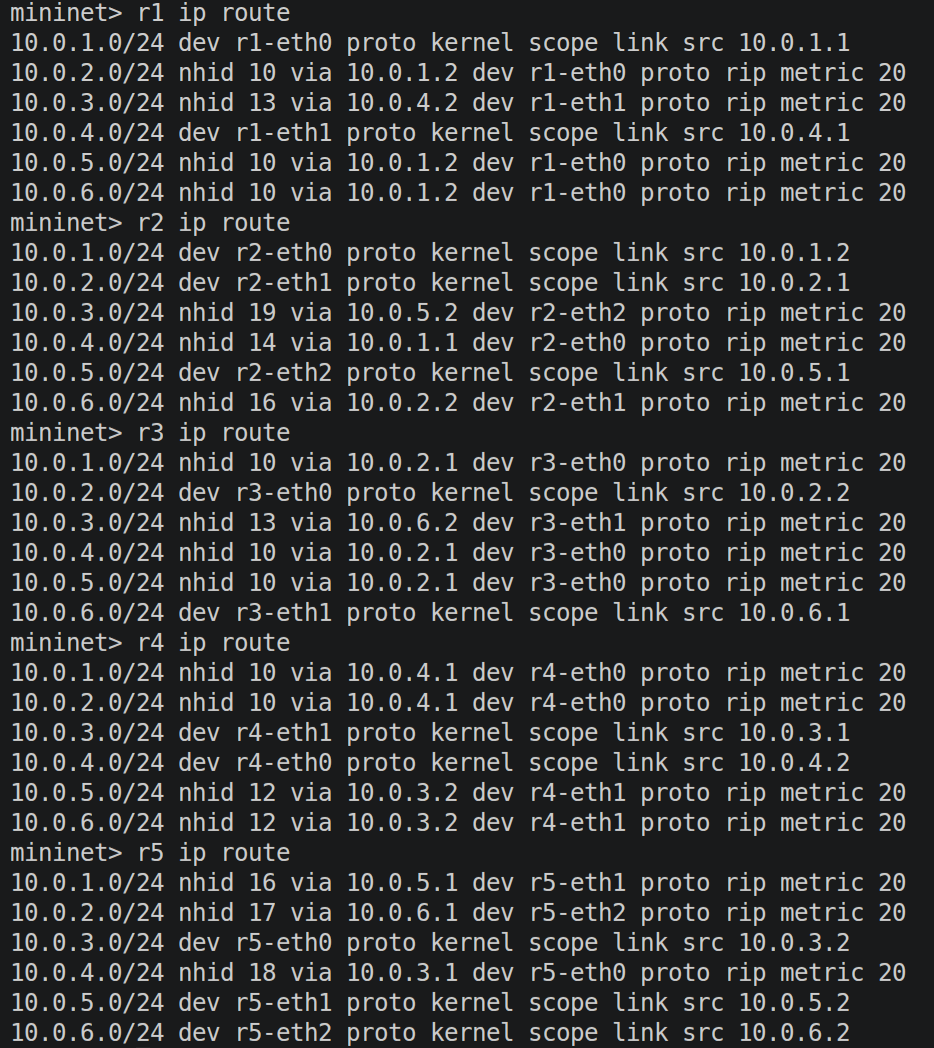
\includegraphics[width =.85\textwidth]{./figures/init_iproute.png}
    \caption{R1-R5初始化路由表}
\end{figure}

\newpage

\subsubsection*{(3) 测试连通性}
从 R1 分别 ping R3 和 R5。
用 R3 在 R3-R5 链路上的接口地址10.0.6.1 以及 R5 在 R4-R5 链路上的接口地址 10.0.3.2 测试。
从连通性测试截图图2中可以看到，两次 ping 测试均显示
\begin{lstlisting}
3 packets transmitted, 3 received, 0% packet loss
\end{lstlisting}

这说明 R1 到 R3、R1 到 R5 均能够正常通信。
R1 虽然并不直接连接 R3 和 R5 的目标接口，但由于 RIP 已经学习到了对应的路由，数据包可以通过动态路由转发到目标网络。
这进一步说明了RIP 路由配置有效。

\begin{figure}[!htbp]
    \centering
    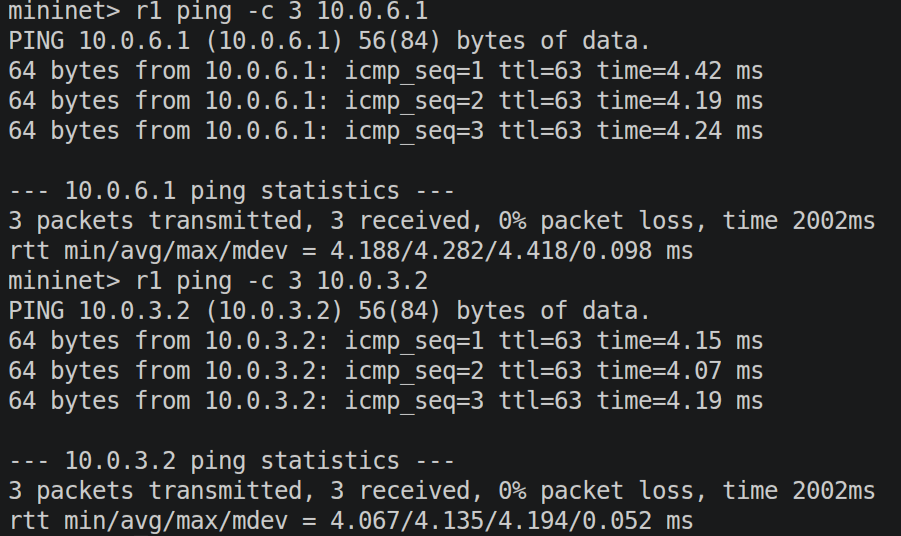
\includegraphics[width =.8\textwidth]{./figures/ping1.png}
    \caption{初始化连通性测试截图}
\end{figure}

\subsubsection*{(4) 断开 R2-R5 链路后的路由更新}
用\texttt{link r2 r5 down}模拟链路故障，断开 R2 与 R5 之间的链路，即网段 10.0.5.0/24 对应的链路失效。
断链后再次查看 R1、R2、R5 的路由表。从截图图3可以观察到明显变化：
\begin{itemize}
    \item R2与R5 的直连路由发生变化：断链前，R2与R5 的路由表中存在R2-R5之间的直连链路\texttt{10.0.5.0/24 dev r2-eth2 proto kernel}，
    断链后，路由表中已经不再显示 \texttt{10.0.5.0/24 dev r2-eth2}，说明 R2-R5 链路已经被成功断开。
    \item R2 到 R5 相关网络的路由发生改变：R2 已不再通过 R2-R5 直连链路到达 R5 方向，而是改为通过 R3 转发： 
    \begin{lstlisting}
        10.0.3.0/24 via 10.0.2.2 dev r2-eth1 proto rip
        10.0.6.0/24 via 10.0.2.2 dev r2-eth1 proto rip    
    \end{lstlisting}
    即路径变为R2 → R3 → R5。
    \item 同理，R5 到 R1、R2 相关网段的路径变为通过 R3 转发：路径变为R5 → R3 → R2 → R1。
\end{itemize}

因此，虽然 R2-R5 链路发生故障，但由于拓扑中仍然存在其他可达路径，RIP 能够重新选择路由，使网络保持连通。

\begin{figure}[!htbp]
    \centering
    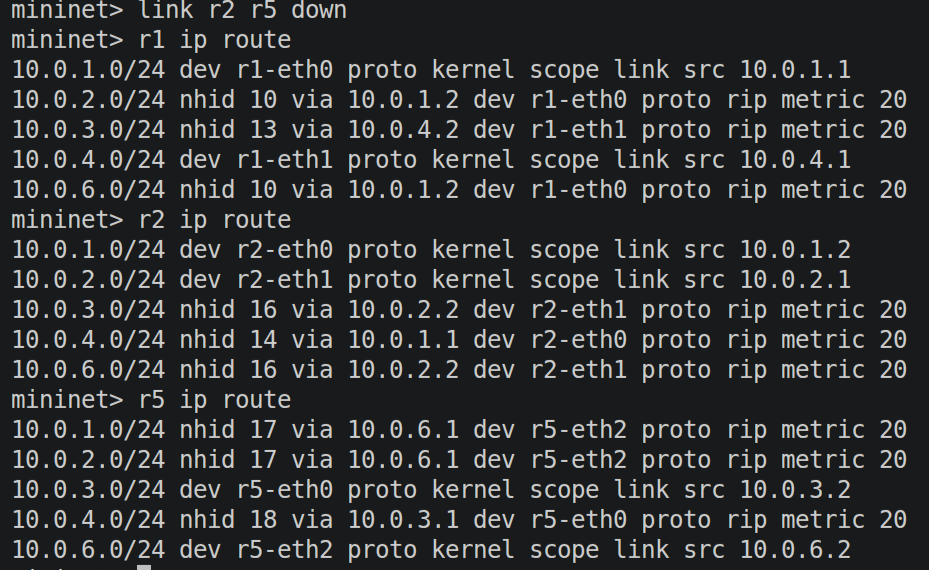
\includegraphics[width =.8\textwidth]{./figures/updated_iproute.png}
    \caption{断链后更新的部分路由表}
\end{figure}


\subsubsection*{(5) 断链后连通性测试}
再次从 R1 测试到 R3 和 R5 的连通性，得到图4。
从测试结果可以看到，两次 ping 仍然显示可达。
这说明 RIP 协议已经根据链路故障重新更新路由表，并选择了新的可用路径。
断链后的连通性测试证明 RIP 已完成重新收敛。

\begin{figure}[!htbp]
    \centering
    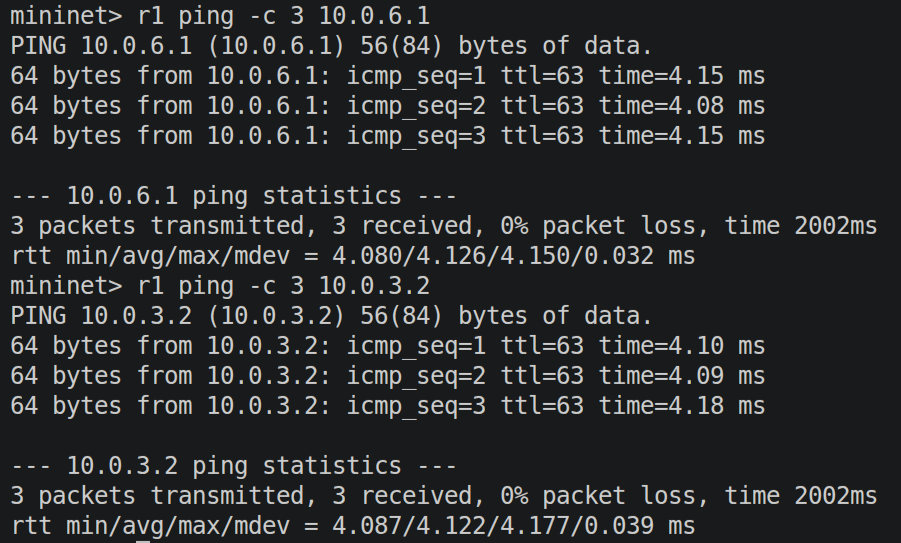
\includegraphics[width =.8\textwidth]{./figures/ping2.png}
    \caption{断链后连通性测试}
\end{figure}

\subsubsection*{(6) 恢复 R2-R5 链路后的路由更新}
用\texttt{link r2 r5 up}恢复R2-R5链路。
从恢复后的路由表截图图5可以看出，R2 和 R5 的直连网段 10.0.5.0/24 已经重新出现，说明 R2-R5 链路已经恢复成功。
同时，一些其他部分的路由又重新通过对R2-R5 链路的学习选择，例如R5 到 R1 方向的路由：
\begin{lstlisting}
10.0.1.0/24 via 10.0.5.1 dev r5-eth1 proto rip
\end{lstlisting}
所表示的路径为R5 → R2 → R1，R2 和 R5 重新拥有 10.0.5.0/24 的直连路由。

\qquad 

\subsection*{3. 分析 RIP 协议在链路故障时的收敛时间及路由环路避免机制}
\subsubsection*{(1) RIP收敛时间分析}
在本次实验中，初始状态下所有链路正常，五台路由器通过 RIP 相互交换路由信息，最终每台路由器都学习到了所有非直连网段的路由。

当 R2-R5 链路断开后，R2 和 R5 失去了 10.0.5.0/24 的直连路由。随后 RIP 根据其他邻居通告的信息重新选择路径。例如 R2 可以通过 R3 到达 R5，R5 也可以通过 R3 到达 R2 和 R1。
因此，网络并未完全中断，而是经过短暂收敛后恢复正常转发。

当 R2-R5 链路重新连接后，R2 与 R5 再次恢复直连关系，并重新通过 RIP 通告该链路。其他路由器接收到新的路由信息后，再次更新自己的路由表，使路由状态回到接近初始状态。

\subsubsection*{(2) 路由环路避免机制}
RIP 作为一种距离向量协议，在链路故障时可能出现路由环路或“计数到无穷”问题。为了缓解这些问题，RIP使用以下机制：
\begin{itemize}
    \item 最大跳数限制：RIP 规定最大跳数为 15，跳数达到 16 时表示不可达，限制错误路由无限传播。
    \item 水平分割性质：路由器不会把从某个接口学习到的路由再从同一个接口通告回去，从而减少两个路由器之间形成简单环路的可能。
    \item 当某条路由失效时，路由器会向邻居通告该路由不可达，加快对错误路由的清除。
    \item 当链路状态发生变化时，路由器不必完全等待周期性更新，而是可以主动向邻居发送更新信息。
\end{itemize}

在本实验中，断开 R2-R5 链路后，RIP 能够重新选择 R2-R3-R5 或 R1-R4-R5 等替代路径，说明路由器之间完成了动态更新，
没有出现明显的长期路由环路。

\subsection*{4. 思考题解答}
Q: 如果将所有链路代价改为非对称值（如 R1-R2=1，R2-R1=5），RIP 协议能否正
常工作？

A: 可能无法正常工作。RIP 本身不适合精确处理非对称链路代价。
RIP 的度量标准主要是跳数，而非链路带宽、延迟或方向性代价。
如果网络中存在非对称链路代价（如 R1-R2=1，R2-R1=5），那么实际网络代价具有方向性。
但是 RIP 的默认跳数度量无法准确表达这种方向差异，因此无法选择最低代价路径。

因此，RIP 只能维持基本连通性，不能很好地根据非对称链路代价选择最优路径。
\end{document}